% https://tex.stackexchange.com/questions/56254/how-to-design-a-3d-donut-pie-chart-with-pgf-plot
% CAUTION: Please do not run this script. (3d-charts with PGF) ;-)
\documentclass[tikz]{standalone}
\usetikzlibrary{fadings}
\begin{document}
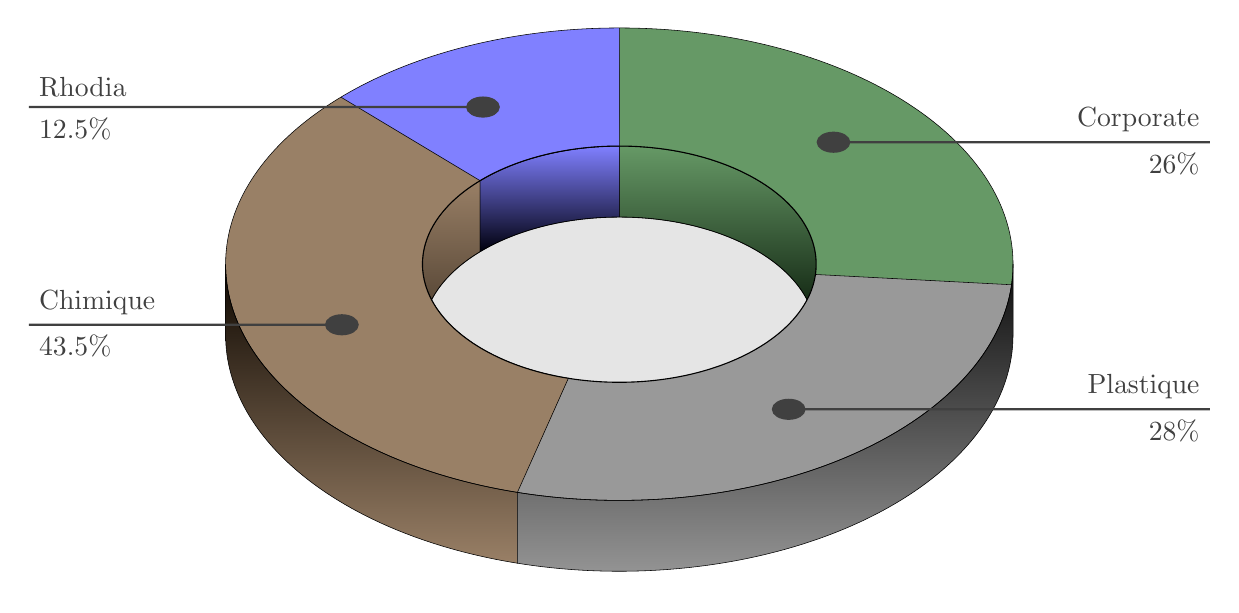
\begin{tikzpicture}[fading style/.style	=	{preaction={fill=#1,opacity=.8,
														path fading	=	circle with fuzzy edge 20 percent}}]
	
	\begin{scope}[xscale=5,yscale=3]
		\path[fading style=black,transform canvas={yshift=-40pt}] (0,0) circle (1cm);
		\fill[gray](0,0) circle (0.5cm);
		\path[fading style=white,transform canvas={yshift=-16mm}] (0,0) circle (0.65cm);
		\draw[yshift=-3mm](0,0) circle (0.5cm);

		\shadedraw[top color=green!20!gray,,bottom color=green!5!black,draw=black,very thin]
			(90:0.5cm)--++(0,-3mm) arc(90:-5:0.5cm)--++(0,3mm)  arc(-5:90:0.5cm)--cycle;
		\shadedraw[top color=orange!20!gray,bottom color=orange!5!black,draw=black,very thin]
			(-105:0.5cm)--++(0,-3mm) arc(-105:-225 :0.5cm)--++(0,3mm)  arc(-225:-105:0.5cm)--cycle;
		\shadedraw[top color=blue!50!white,,bottom color=blue!5!black,draw=black,very thin]
			(135 :0.5cm)--++(0,-3mm) arc(135:90:0.5cm)--++(0,3mm)  arc(90:135:0.5cm)--cycle;

		\begin{scope}[draw=black,thin]
			\fill[green!20!gray](90 :0.5cm)--(90:1cm) arc(90:-5:1cm)--(-5:0.5cm) arc(-5:90 :0.5cm);
			\fill[white!20!gray](-5 :0.5cm)--(-5:1cm) arc(-5:-105 :1cm)--(-105:0.5cm) arc(-105:-5:0.5cm);
			\fill[orange!20!gray](-105:0.5cm)--(-105:1cm) arc(-105:-225 :1cm)--(-225:0.5cm)	arc(-225:-105:0.5cm);
			\fill[blue!50!white](135:0.5cm)--(135 :1cm) arc(135:90:1cm)--(90:0.5cm) arc(90:135:0.5cm);
		\end{scope}
		
		\draw[thin,black](0,0) circle (0.5cm);

		\shadedraw[bottom color=orange!20!gray,top color=orange!5!black,draw=black,very thin]
			(-180:1cm) --++(0,-3mm) arc (-180:-105 :1cm) -- ++(0,3mm)  arc (-105 :-180  :1cm) -- cycle;
		\shadedraw[bottom color=white!20!gray,top color=white!5!black,draw=black,very thin]
			(-105:1cm) --++(0,-3mm) arc (-105:0 :1cm) -- ++(0,3mm)  arc (0 :-105  :1cm) -- cycle;

		\draw[very thin] (90:0.5cm) -- (90:1cm)	(-5:0.5cm) -- (-5:1cm)	(-105:0.5cm) -- (-105:1cm)	(135:0.5cm) -- (135 :1cm)	(0,0) circle (1cm)	(90:0.5cm) arc (90:135:0.5cm);
		\coordinate (left border) at (1.5cm,0cm);
		\coordinate (right border) at (-1.5cm,0cm);
		\coordinate (l1) at (43.5:0.75 cm);
		\coordinate (l2) at (-55:0.75 cm);
		\coordinate (l3) at (117.5:0.75 cm);
		\coordinate (l4) at (-160:0.75 cm);

		\begin{scope}[lab/.style={gray!50!black,thick,draw}]
			\fill[lab] (l1) circle(.4mm) -- (l1-| left border) node[anchor=south east] {Corporate}
				node[anchor=north east] {26\%};         
		\fill[lab] (l2) circle(.4mm) -- (l2-| left border)  node[anchor=south east] {Plastique}
				node[anchor=north east] {28\%}; 
		\fill[lab] (l3) circle(.4mm) -- (l3-| right border) node[anchor=south west] {Rhodia}
				node[anchor=north west] {12.5\%};         
		\fill[lab] (l4) circle(.4mm) -- (l4-| right border) node[anchor=south west] {Chimique}
				node[anchor=north west] {43.5\%}; 
		\end{scope}
	\end{scope} 
\end{tikzpicture}    
\end{document}    